\section{Methodology}

\begin{frame}
\begin{center}
     	\huge Methodology
     \end{center}
\end{frame}

\begin{frame}
\frametitle{The Approach}
\begin{figure}
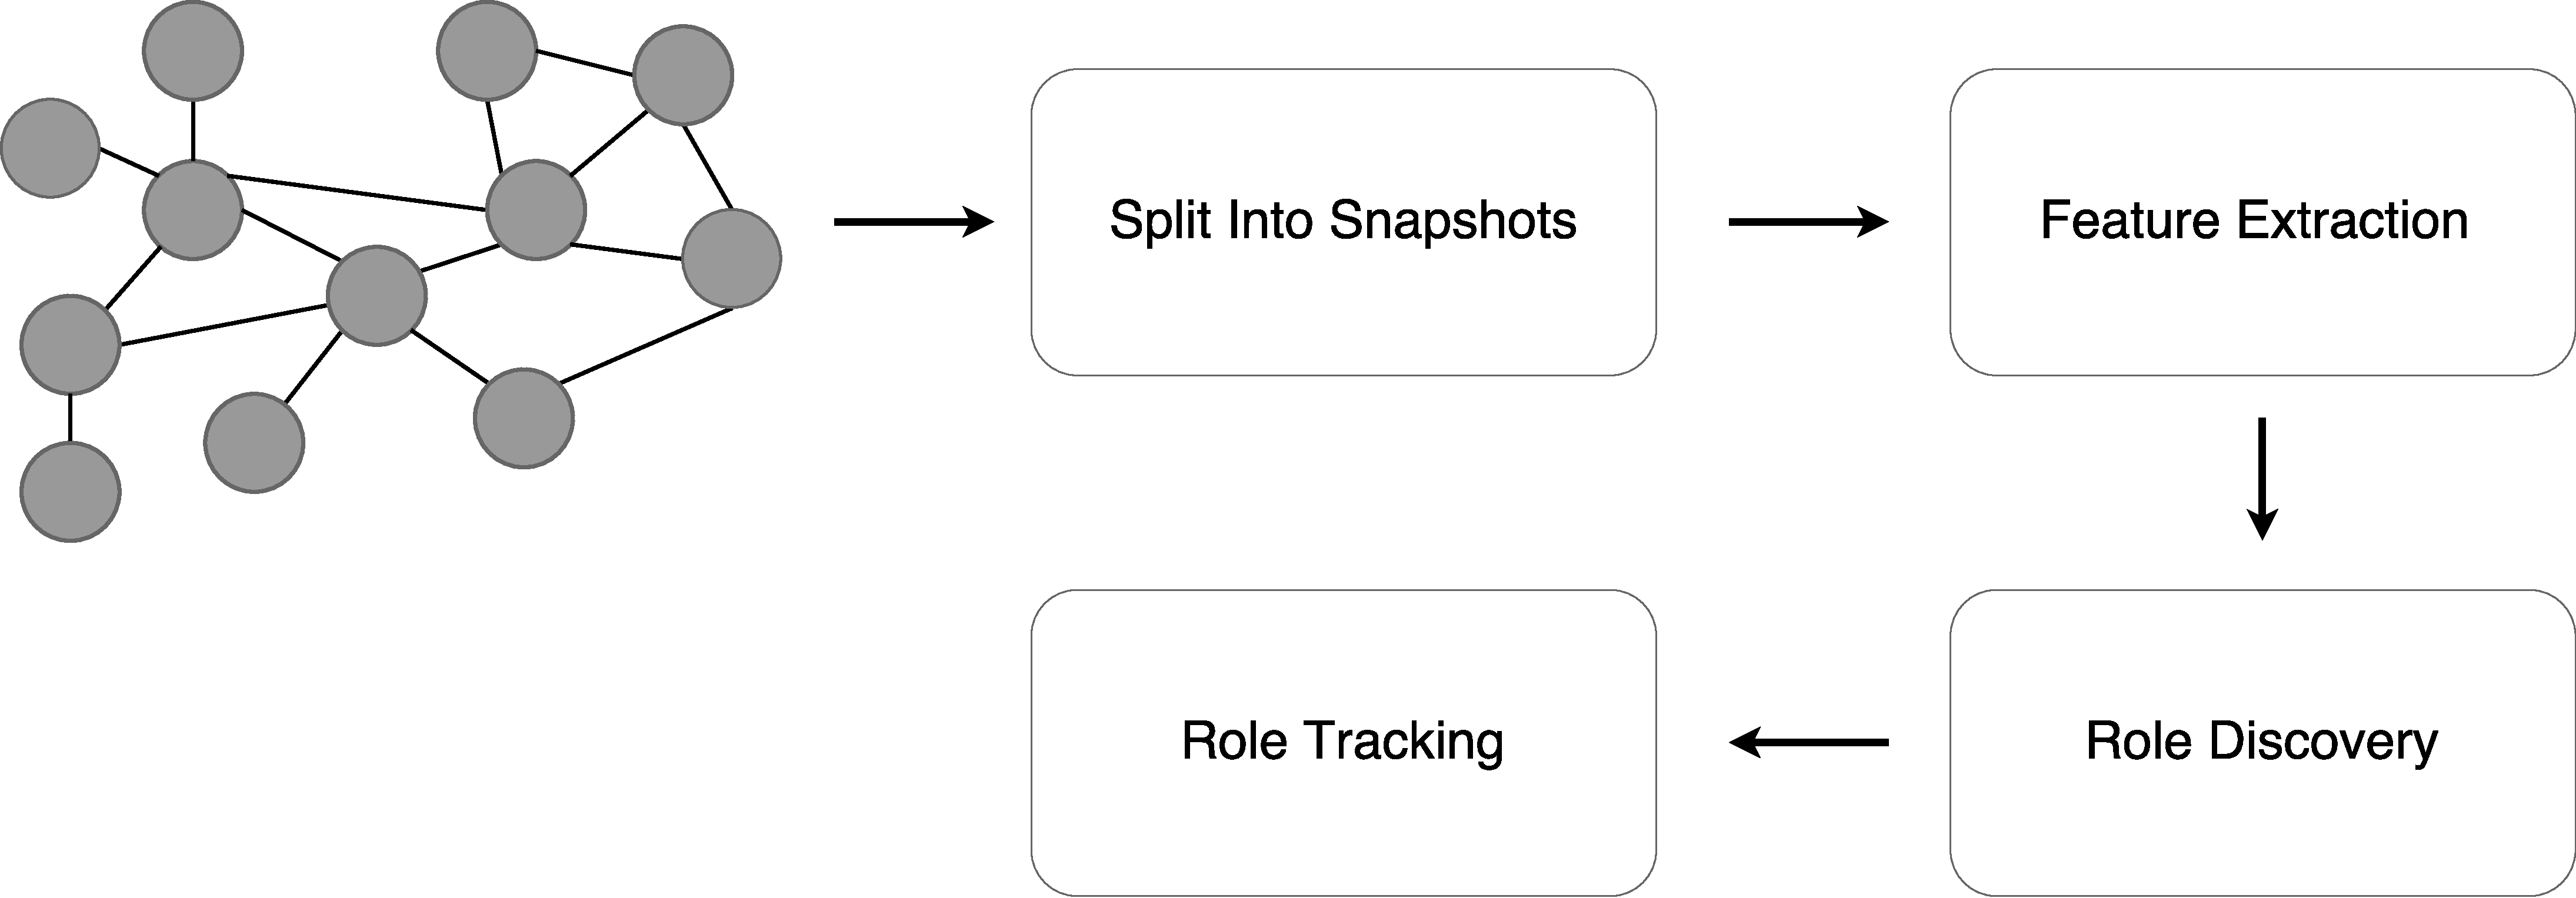
\includegraphics[scale=0.1]{graphics/setup.pdf}
\end{figure}
\end{frame}

\begin{frame}
\frametitle{Data Format}
\begin{columns}
	\begin{column}{0.4\textwidth}
			\begin{itemize}
				\item Facebook - wall posts 
				\item Scratch - ?
			\end{itemize}
			Directed, timestamps.
		\end{column}
		\begin{column}{0.6\textwidth}
			\begin{figure}
				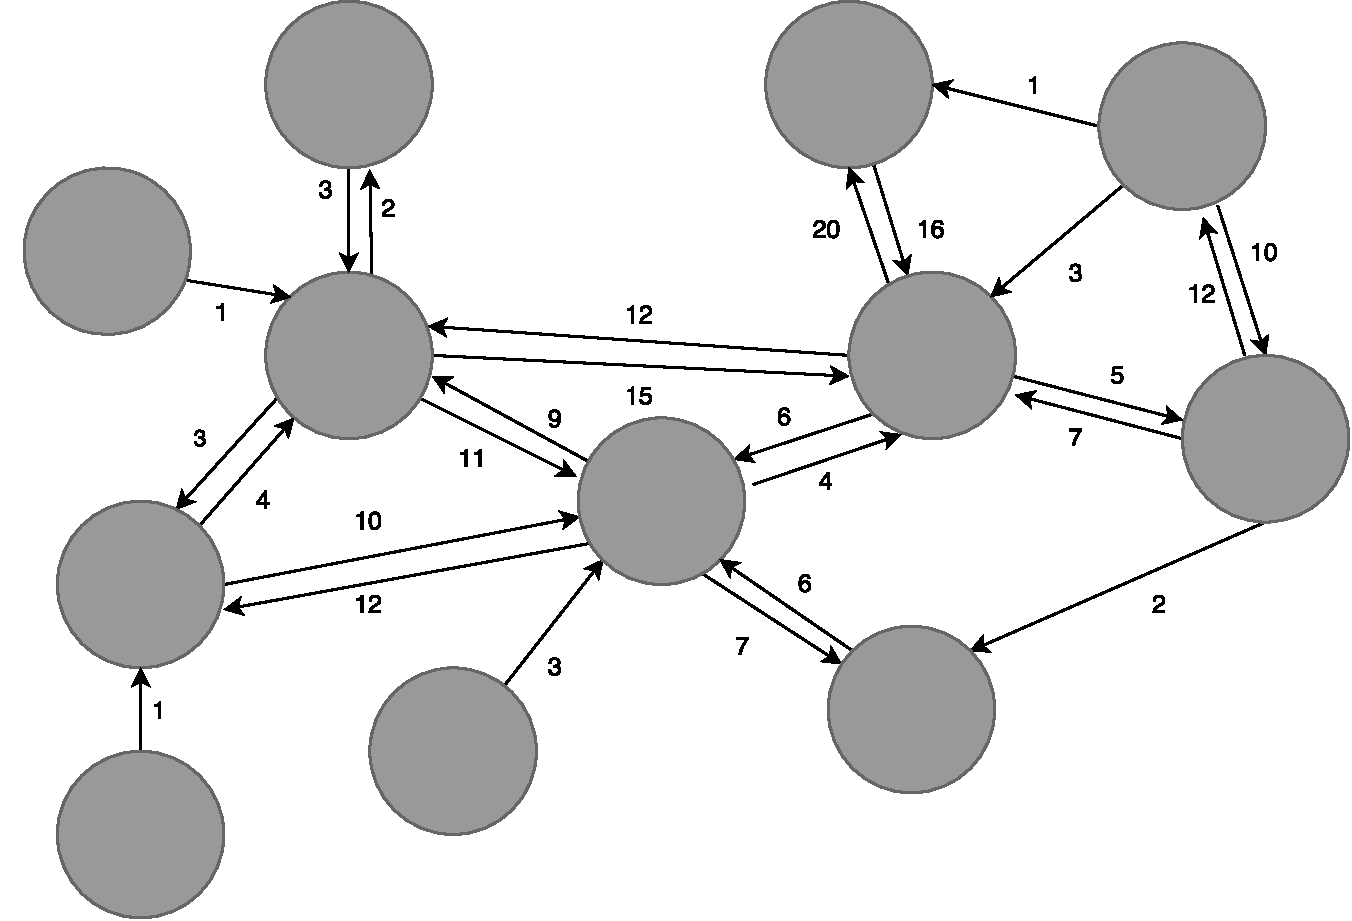
\includegraphics[scale=0.27]{graphics/directed_network.pdf}
			\end{figure}
		\end{column}
	\end{columns}
\end{frame}

\begin{frame}
\frametitle{Snapshot Split-up}
\end{frame}

\begin{frame}
\frametitle{Feature Selection}
\end{frame}

\begin{frame}
\frametitle{Feature Example}


\begin{columns}
		\begin{column}{0.5\textwidth}
			\begin{figure}
				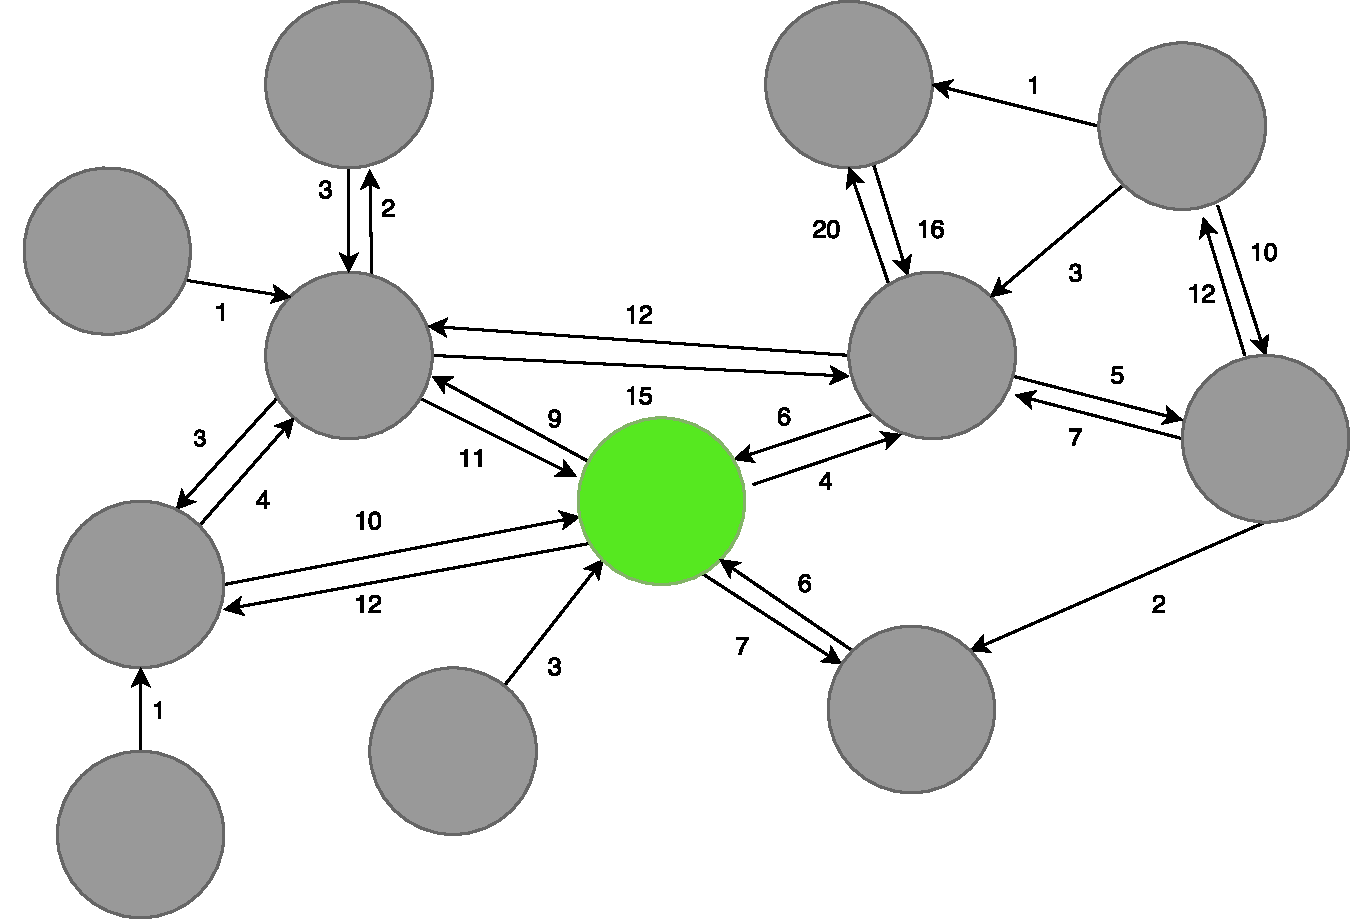
\includegraphics[scale=0.27]{graphics/directed_network_example.pdf}
			\end{figure}
		\end{column}
		\begin{column}{0.5\textwidth}
			\begin{table}
				\begin{tabular}{|l|l|}
				\hline
					In-degree				& 5		\\ \hline
					Out-degree				& 4		\\ \hline
					Weighted in-degree		& 36	\\ \hline
					Weighted out-degree		& 32	\\ \hline
					Reciprocity				& 		\\ \hline
					New activity			& 0		\\ \hline
					Social strategy			& 0		\\ \hline
					Betweenness centrality	& 		\\ \hline
					PageRank				& 		\\ \hline
					Weighted PageRank		& 		\\ \hline
					Transitivity			& 		\\ \hline
					Weighted transitivity 	& 		\\ \hline
			\end{tabular}
			\end{table}
		\end{column}
	\end{columns}

\end{frame}

\begin{frame}
\frametitle{Role Assignment}
NMF
NNDSVD
feature size of 6 (based on RMSE)
\end{frame}

\begin{frame}
\frametitle{Tracing Roles}
The sim between snapshots. 
\end{frame}